\documentclass{article}

% PACKAGES
\usepackage[utf8]{inputenc}
\usepackage{blindtext}
\usepackage{multicol}
\setlength\columnsep{0.35in} % sets space between columns

\usepackage{amsmath}
\usepackage{amsfonts}
\usepackage{amssymb}
\usepackage{amsthm}
\usepackage{gensymb}
\usepackage{commath}
\usepackage{esdiff} % Differentiation
\usepackage{marvosym, wasysym} % More symbols
\usepackage{mathtools}

\usepackage{graphicx} % images
\usepackage{wrapfig} % text wrapping
\usepackage{scalerel} % Scaling
\usepackage{pdfpages} % import pdf
\usepackage{fancyhdr} % fancy headers and footers
\usepackage{float} % floating tables and figures

\PassOptionsToPackage{usenames, dvipsnames}{color}
\usepackage{color}

\PassOptionsToPackage{hyphens}{url}
\usepackage[hyperfootnotes=false,hidelinks]{hyperref}

\usepackage{comment} % allows using \begin{comment} to do block comments

\usepackage[12pt]{extsizes} % allows larger font sizes (defaulting to 12 pt)
\usepackage[left=0.565in,right=0.565in,top=0.935in,bottom=0.935in]{geometry} % custom margins

\newcommand{\ubar}[1]{\underaccent{\bar}{#1}}
\newcommand\ddfrac[2]{\frac{\displaystyle #1}{\displaystyle #2}} % Allows for "uncramped" fractions
\DeclareMathOperator*{\gint}{\scalerel*{\mathnormal{\pi}}{\big(}} % lowkey idk why this exists

\usepackage{tcolorbox} % colored text boxes
\usepackage{tikz} % diagrams, plots, illustrations, etc using raw LaTeX
\usetikzlibrary{positioning, calc} % additional tikz libraries

\usepackage{accents} % manipulating accent positioning
\usepackage{indentfirst} % indent first paragraph
\usepackage{dirtytalk} % typesetting quotes using \say{...}

\usepackage{lastpage} % allows reference to num of pages (i.e. page X of Y)

\usepackage{tocloft} % table of contents
\renewcommand{\cftsecleader}{\cftdotfill{\cftdotsep}}

\usepackage{setspace} % line spacing control
\setstretch{1.04} % custom line spacing of 1.04

% DOCUMENT
\begin{document}
\pagestyle{fancy}
\lhead{Eagle's $\sqrt{-1}$, 4\textsuperscript{th} Edition}
\rhead{May 2025}

% TITLE PAGE
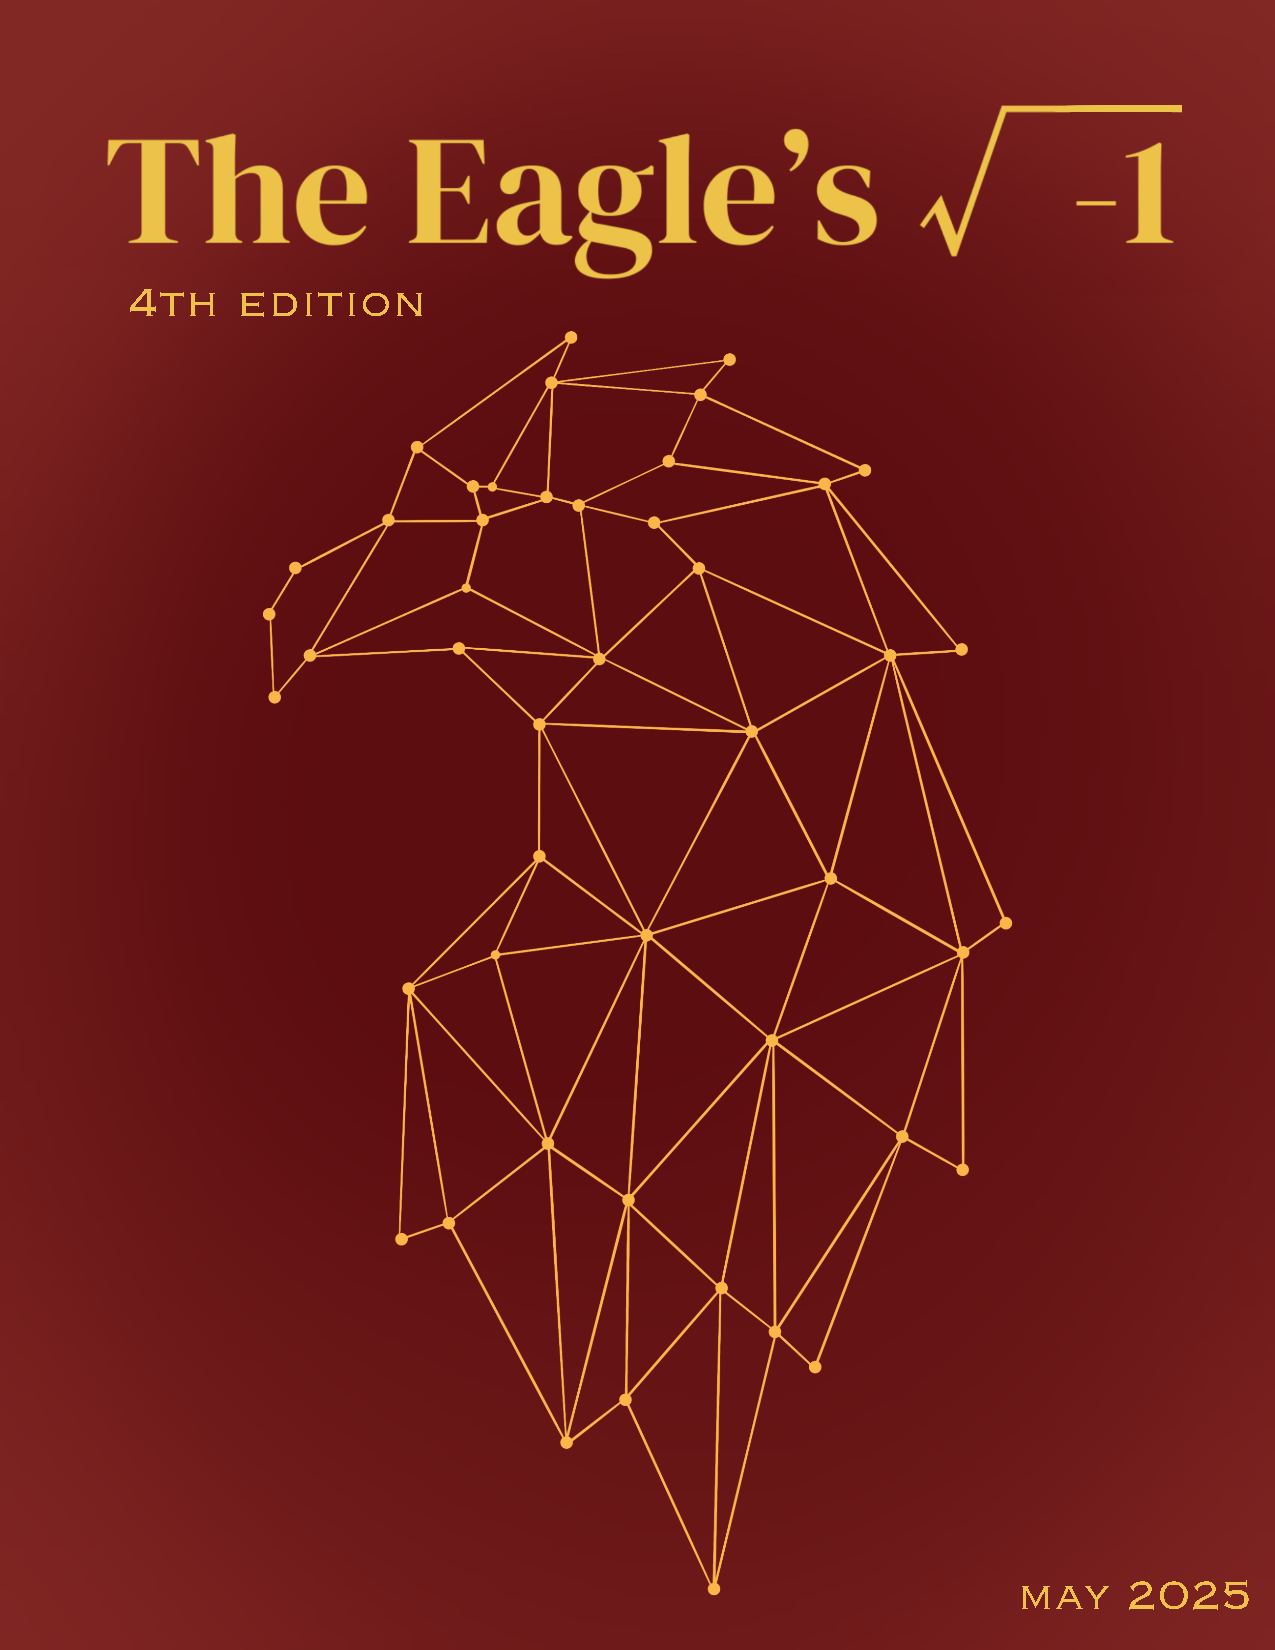
\includepdf{front}

% TABLE OF CONTENTS
\renewcommand*\contentsname{\textbf{Table of Contents}}
\tableofcontents
\thispagestyle{fancy}
\vspace{60pt}
\pagebreak

% ARTICLES
\begin{multicols}{2}

\section*{$\pi + e =$ ?}
\addcontentsline{toc}{section}{\texorpdfstring{$\pi + e$}{pi + e} = ? by Ankita Varigonda '25}
\noindent\textbf{Ankita Varigonda '25}
\medbreak

$\pi$, the constant that relates the diameter of a circle to its circumference, is a number that arises naturally. For centuries, we have discovered numerous methods that all lead to this singular value: approximations using polygons with an increasing number of sides, the Leibniz formula, and more. The number $e$ occupies a similar position. Like $\pi$, $e$ appears in unlikely places and describes growth in the natural world. There are also almost an endless number of fields in which these constants appear, evoking the thought that they are fundamentally related to our universe. Numbers such as these are placed in their own category and are called transcendental numbers. Both of these constants have an infinite number of digits, and their decimal expansions do not follow a pattern, but this is not unique, as many irrational numbers such as $\sqrt{2}$ have the same properties. Then, what makes $\pi$ and $e$ transcendental?

\subsection*{Algebraic Numbers}

We must first discuss algebraic numbers before defining transcendental numbers. Take a number $x$. If you can perform a sequence of additions, subtractions, multiplications, and exponentiations of natural numbers (positive integers) on $x$ such that the combination of these operations results in zero, then $x$ is an algebraic number. Considering this definition, numbers such as $3$, $\frac{1}{5}$, $\sqrt{3}$, and even $i$ are algebraic numbers (see if you find the sequence of operations needed to reduce these numbers!). From here, another definition of algebraic numbers arises, numbers that are expressed as a root of a polynomial with rational coefficients. The set of algebraic numbers turns out to be closed under both addition and multiplication, so any sum or product of algebraic numbers is another algebraic number.

Mathematicians took this a step further and were curious about numbers that did not satisfy these conditions. Thus, the classification of transcendentals arose to be the opposite of algebraic numbers: numbers that cannot exist as the root of a polynomial with rational coefficients.

\subsection*{Transcendentals through History}

In the 1870s, the French mathematician Charles Hermite was able to prove that $e$ is not algebraic and thus transcendental in a proof by contradiction. At last, there was confirmation that $e$ belonged to the elusive group of transcendentals. Based on Hermite’s process, in 1882, Ferdinand von Lindemann proved that for any algebraic number $a$ that was not zero, $e^{a}$ would be transcendental. Finally, using Euler’s Equation, this was extended to $\pi$, as informally proved below:

\begin{proof}
We want to prove that $\pi$ is transcendental, so for a proof by contradiction, we must assume that $\pi$ is algebraic. Euler’s equation can be rewritten: $e^{i\pi} + 1 = 0$, thus $e^{i\pi} = -1$. $i$ is an algebraic number since it is a solution to the equation $x^{2} + 1 = 0$. From our assumption that $\pi$ is algebraic and the fact that algebraic numbers are closed under multiplication, $i\pi$ must also be an algebraic number. Considering Lindemann’s result, since $i\pi$ is algebraic, $e^{i\pi}$ must be transcendental. However, $e^{i\pi} = -1$, which is not transcendental, so our assumption must be false, meaning $\pi$ is not algebraic and thus must be transcendental.
\end{proof}

Finally, it had been proved that $\pi$ was also transcendental. Furthermore, in 1934, a major breakthrough occurred when both Gelfond and Schneider independently proved the Gelfond-Schneider theorem, stating that $a^{b}$ is transcendental for an algebraic number a such that $a \neq 0, 1$ and any algebraic, irrational number $b$. This led to some interesting results, such as the number $2^{\sqrt{2}}$, the Gelfond-Schneider constant, which was proved to be transcendental.

\subsection*{The Unsolved Pie}

But what about $\pi + e$? We would think that the sum of two of the most known constants would have a well-defined answer, but the truth is, the problem still remains open. We cannot assume that because two numbers are transcendental, expressions involving them are transcendental as well. Simply, if we think of $e^{\ln{3}}$, which is equal to $3$, it is evident that $\ln{3}$ must be transcendental based on Lindemann’s proof. This means that transcendental numbers raised to the power of each other have the potential to be integers. Similarly, it is unknown whether their sums could result in algebraic numbers.

Numerous attempts have been made to find whether expressions related to both numbers are transcendental, and there have been few successes. $e^{\pi}$ was proved to be transcendental using Gelfond-Schneider theorem, but $\pi^{e}$, $\pi e$, $e^{e}$, and many more expressions are still unknown. Yet mathematicians are relentless, and even today, there are results bringing us closer to a breakthrough. Someday, we may have a definitive answer to what $\pi + e$ really is.

\section*{Understanding Volume with Integration}
\addcontentsline{toc}{section}{Understanding Volume with Integration by Jiko Chatterjee '27}
\noindent\textbf{Jiko Chatterjee '27}
\begin{center}
    \includegraphics[width=5cm]{Jiko1.png}
\end{center}
\subsection*{Introduction}
If you are reading this, you probably know that the volume of a sphere is given by the formula $\frac{4}{3}\pi{r}^{3}$. But do you know where this formula comes from? Why is it $\frac{4}{3}$ and not another number? And what if the shape in question isn’t a sphere---how would we determine its volume? That’s what I’m going to show you.

\subsection*{How does it work?}

To find the volume of a 3D shape, we use a method called \textbf{integration} along with \textbf{cross-sections}. Imagine you have a ball or any other 3D shape (like a strawberry). If you were to slice it into many thin layers of equal thickness, each slice would be a cross-section. These cross-sections are much easier to calculate than the volume of the entire shape.

The key idea is that as the slices become thinner, the sum of their volumes (\textbf{area of the cross-section} $\times$ \textbf{thickness}) gets closer and closer to the actual volume of the shape. Now, you may be wondering “what if the slices have a weird base that is curvy and hard to calculate?” This is where integration is critical. Integration allows you to calculate the area of a region bounded by a curve and the x-axis (or another axis).
\begin{center}
    \includegraphics[width=5cm]{Jiko2.png}
\end{center}
Now, you may be wondering, “How do you calculate the thickness?” To determine the thickness of each slice, we use $dx$, which represents an infinitesimally small change in the variable along the axis of integration. With this method, we arrive at a general approach to solving for volumes:

\begin{equation*}
    V_x = \int_{a}^{b} A(x)dx
\end{equation*}

\subsection*{Volume of a Sphere}

Now, let's answer our original question: How does the formula for the volume of a sphere come to be? A sphere can be graphed by the equation where $x$, $y$, $z$ represent length, width, and height:

\begin{equation*}
    x^2 + y^2 + z^2 = r^2
\end{equation*}

For simplicity, let’s assume $r = 1$ (\textbf{a unit sphere}). This means the center of the sphere is at $(0, 0, 0)$. Thus, $z$ varies from $-1$ to $1$, which defines the bounds of our integral. By solving for $x^2 + y^2$, we get:

\begin{equation*}
    x^2 + y^2 = 1 - z^2
\end{equation*}

The right-hand side represents the square of the radius of a cross-section at a given height $z$. The volume of the sphere is then found by integrating the areas of these circular cross-sections:

\begin{equation*}
    V = \int_{-1}^{1} \pi(1 - z^2)dz
\end{equation*}

Finally, we evaluate the integral:

\begin{equation*}
    V = \left. \pi (z - \frac{z^3}{3})\right\vert_{-1}^{1} = \frac{4\pi}{3}; \ r = 1
\end{equation*}

And there we have it---the formula for the volume of a sphere! Now that you understand the method, you can try applying it to any other shape, such as a cone, and see if you derive their volume formulas as well.
\subsection*{Volume of a Hypersphere}
\begin{center}
    \includegraphics[width=5cm]{Jiko3.png}
\end{center}
Now that you hopefully had more practice, let's find the volume of a unit hypersphere (4-D)!
\subsection*{Geometric Foundations}
The 4D unit hypersphere is defined by the equation:
\begin{equation*}
    x^2 + y^2 + z^2 + w^2 = 1
\end{equation*}
where $(x,y,z,w)$ are coordinates in $4$-dimensional space. Similar to how a $3$D sphere’s cross-sections are $2$D circles at a fixed height $z$, the cross-sections of a hypersphere are $3$D sphere at a fixed point of time $w$. With this we get a radius of $\sqrt{1 - w^2}$, centered at the origin.

Using the same we covered earlier, plugging in $\sqrt{1 - w^2}$ as a radius given by the standard volume formula of the sphere, $\frac{4\pi r^3}{3}$, results in an integral: 
\begin{equation*}
    V(w) = \int_{-1}^{1}(\frac{4\pi}{3}(1 - w^2)^\frac{3}{2})dw
\end{equation*}
Now, by using trig substitutions to evaluate this integral we get the hypervolume of the $4$-dimensional unit hypersphere as:
\begin{equation*}
    \frac{\pi^2}{2}
\end{equation*}
There you have it! Now feel free to brag to your friends that you know the volume of a $4$-D shape!
\section*{Zero Knowledge Proofs}
\addcontentsline{toc}{section}{Zero Knowledge Proofs by Thomas Ha '26}
\noindent\textbf{Thomas Ha '26}
\medbreak

Imagine you're holding a piece of secret information that you need to prove you know---but you can't reveal the secret itself. Sounds like magic, right?

First conceived in the 1980s by researchers Shafi Goldwasser, Silvio Micali, and Charles Rackoff, zero-knowledge proofs (or ZKPs) allow individuals to prove the truth of a statement without revealing any other information. ZKPs can thus be applied to authentication systems, cryptocurrency, voting systems, and even nuclear disarmament.

\subsection*{Definitions}

While there are "formal" definitions for nearly everything explained here, we will define the following terms loosely.

\begin{enumerate}
    \item \textbf{Honesty}: an honest verifier or prover follows the proof protocol properly.
    \item \textbf{Maliciousness}: a malicious prover attempts to convince a verifier that the statement is true even if it is not.
\end{enumerate}

It is rare to encounter a malicious verifier, and in any case, it would not be particularly interesting to discuss, so we will simply ignore that case. In both examples we discuss, both the verifier and prover will be honest. A ZKP must satisfy three properties:

\begin{enumerate}
    \item \textbf{Completeness}: if the statement is true, then an honest verifier will be convinced of its truthfulness by an honest prover.
    \item \textbf{Soundness}: if the statement is false, then an honest verifier will (in most cases) not be convinced of its truthfulness by a malicious prover.
    \item \textbf{Zero-knowledge}: if the statement is true, then a verifier cannot learn anything other than the statement is true.
\end{enumerate}

\subsection*{Where's Waldo?}

In this example, a prover wants to prove to the verifier that they know where Waldo is on a \textit{Where's Waldo?} page without revealing where it is to the verifier.

The proof requires a cardboard sheet at least double the size of the page in both directions. The prover then cuts a small hole the exact size and shape of Waldo in the center of the board. Then, the prover places the cardboard sheet over the page such that Waldo is in the hole.

The verifier can now see Waldo through the hole, proving that the prover knows where Waldo is. However, since the verifier cannot see any other part of the page, the prover has not revealed any information about Waldo's location.

This proof therefore satisfies the three requirements for a zero-knowledge proof. The \textit{completeness} of the proof is obvious: if the prover knows where Waldo is, they will always be able to place the cardboard sheet such that Waldo is visible. The \textit{zero-knowledge} aspect is also obvious.

Recall that when defining \textit{soundness}, however, we used the phrase "in most cases." A malicious prover who \textit{does not} know where Waldo is can \textit{guess} where to place the cardboard sheet. In nearly every case the malicious prover will fail, but there is a slim chance that the prover will succeed. This demonstrates the fact that ZKPs are \textbf{probabilistic} rather than \textbf{deterministic}. If a prover uses a ZKP to show that a statement is true (possibly repeating it several times, as we will see later), it is overwhelmingly likely---but not guaranteed---to be true: the prover could be malicious and could have simply been lucky.

\subsection*{Hamiltonian Cycles}

In this scenario, there is a large graph $G$. Peter, the prover, knows a \textbf{Hamiltonian cycle} for $G$.

\begin{itemize}
    \item A graph consists of an arbitrary number of vertices connected by edges, similar to a subway map.
    \item A Hamiltonian cycle of a graph is a \textbf{cycle} that visits every vertex in the graph exactly once.
    \item A cycle is a path (or sequence of vertices) where the first and last vertices in the path are identical---you end up where you started.
\end{itemize}

For a large enough graph, it becomes computationally infeasible to compute a Hamiltonian cycle, since the fastest algorithm to compute one has time complexity $O({N}^{2}{2}^{N})$, or exponential: essentially, as the size increases linearly, the time needed to compute a Hamiltonian cycle grows exponentially. Something computationally feasible must have polynomial time complexity or less.

Victor, the verifier, knows $G$ but not the cycle; Peter needs to prove to Victor that he knows the cycle without directly showing him the cycle. To do this, they repeat the following process several times:

\begin{itemize}
    \item Peter creates $H$, a graph which is isomorphic to $G$ (so $H$ is functionally equivalent to $G$ except that the vertices have different names). More precisely, he applies a bijective function $f: V(G) \rightarrow V(H)$, and any two vertices $u$ and $v$ in $G$ are adjacent if and only if $f(u)$ and $f(v)$ are adjacent in $H$. It is trivial to translate a Hamiltonian cycle between isomorphic graphs given the bijective function, so if Peter knows a cycle for $G$, he must know one for $H$.
    \item Peter commits to $H$; in other words, he can no longer alter $H$, but Victor cannot find out any information about $H$. To do this, he first numbers each vertex of $H$. Then, for each edge of $H$, he writes down the two vertices connected by the edge on a piece of paper---a different paper for each edge. He finally places all the pieces of paper face-down on a table.
    \item Victor then chooses one of two questions to ask Peter.
    \begin{enumerate}
        \item He can ask Peter to show him the isomorphism between $G$ and $H$.
        \item He can ask Peter to show him a Hamiltonian cycle in $H$.
    \end{enumerate}
    \item If Peter is asked to show the isomorphism, he turns over all the pieces of paper and reveals the bijection $f$ that he used to translate the vertices of $G$ onto $H$. Victor can thus verify the isomorphism.
    \item If Peter is asked to show the Hamiltonian cycle, he translates the Hamiltonian cycle from $G$ to $H$ and \textit{only} turns over the edges of the cycle. Victor can thus check that $H$ contains a Hamiltonian cycle.
\end{itemize}

This proof is \textit{complete} because if Peter knows a Hamiltonian cycle in $G$, then he can satisfy Victor's demand for either the isomorphism between $G$ and $H$ or a Hamiltonian cycle in $H$ (proving he knows one in $G$).

This proof is \textit{sound} because if Peter \textit{does not} know a Hamiltonian cycle in $G$, he has a maximum $50\%$ chance of successfully fooling Victor each round. Peter can guess which question Victor will ask and then generate $H$ accordingly to either be isomorphic to $G$ or to have a Hamiltonian cycle (in which case it would be unrelated to $G$). If Peter does not know a Hamiltonian cycle for $G$, he cannot do both. With random guesses, he has a ${2}^{-n}$ chance of fooling Victor after $n$ rounds---realistically impossible, since at $n=10$ rounds his odds would be less than $0.1\%$.

This proof is \textit{zero-knowledge} because, in each round, Victor learns \textit{either} the isomorphism \textit{or} the cycle in $H$. Since he would need both to figure out the cycle in $G$ and since $H$ is distinct in each round, he will never be able to find out the Hamiltonian cycle in $G$.

\section*{Prisoners and Poisonings}
\addcontentsline{toc}{section}{Prisoners and Poisonings by Zoe Guo '27}
\noindent\textbf{Zoe Guo '27}
\medbreak

In a kingdom far, far away, a king is celebrating his birthday with a big feast. He invites all $1000$ of his loyal subjects, and asks them each to bring a bottle of wine as a birthday gift. Every subject complies, and the king is very happy to be receiving $1000$ bottles of fine wine. However, on the eve of the feast, the king is notified that one of his subjects has put a poison in one of the bottles. Unfortunately, none of the wine bottles are out of the ordinary, and the king doesn’t want to waste all of his gifts by pouring his wine out. Suddenly, the king remembers that he is keeping $10$ cruel criminals in his dungeon, and he decides to use them as taste testers to determine which bottle is poisonous, and which is not. How should the king distribute the wine bottles to his prisoners so that he can pinpoint where the poison is?

First, the king tries to solve the problem by giving each prisoner 100 bottles. If he were to tell each prisoner to drink from their bottles, he could at least figure out which of the $10$ groups contains the poison. Then, the king would only have to throw away $\frac{1}{10}$ of his wine. Sounds pretty good, right? But what if there was a way for the king to save all $999$ bottles of not-poisoned wine?

What the king should do is assign each prisoner a number from $1-10$, and assign each bottle a number $0-999$. Then, for prisoner $n$, he should ask the prisoner to drink $2^{n-1}$ bottles, then skip $2^{n-1}$ bottles. For example, prisoner 1 will drink from every other bottle (bottles $0$, $2$, $4$, etc.), prisoner 2 will drink from every two bottles ($0$, $1$, $4$, $5$, $8$, $9$, etc.), prisoner 3 will drink from every four bottles ($0$, $1$, $2$, $3$, $8$, $9$, etc.). In this way, every single wine bottle will have a unique combination of prisoners drinking from it. Bottle $\#0$ will be drunk by all the prisoners, bottle $\#1$ will be drunk by every prisoner except for prisoner $1$, and bottle $\#100$ will be drunk by everyone except prisoners $3$, $6$, and $7$. So if a certain group of prisoners dies, the king can easily use their assigned numbers to calculate which of the bottles drunk contained the poison.

But how does this method work? The answer lies within the powers of two assigned to each prisoner, or, in other words, binary! Let’s give each prisoner a value, based on whether or not they are alive a day after drinking the wine. They are equal to 1 if alive, and $0$ if dead. In this way, we can see the pattern: if all prisoners except $\#2$, $\#4$, and $\#7$ become sick, then the sequence (from prisoner $\#10$ to prisoner $\#1$) is $0001001010$, or the base-$10$ number $74$. This means that bottle $\#74$ contained the poison (because it is the unique bottle that all three prisoners didn’t drink from). What about if all prisoners except for $\#5$ get poisoned? Then the sequence is $0000010000$, or bottle $\#16$. Aha — the math proves the king isn’t doomed after all!

\section*{Introduction to Graph Theory and the Handshaking Lemma}
\addcontentsline{toc}{section}{Introduction to Graph Theory and the Handshaking Lemma by Emma Liu '26}
\noindent\textbf{Emma Liu '26}

\subsection*{What is Graph Theory?}
Graph theory is the study of mathematical structures called \textit{graphs}, which consist of a set of \textit{vertices} (also referred to as \textit{nodes}) connected by \textit{edges}. The formal mathematical definition defines a graph as a pair $(V, E)$, where $V$ is the set of vertices and $E$ refers to the set of edges. Every element $e\in E$ is a set $\{u, v\}$ such that $u\neq v$ and $u$ and $v$ are vertices in the set $V$. 

\begin{center}
    \includegraphics[width=5cm]{graph (1).png}
    
    A simple example of a graph
\end{center}

How are graphs applicable to the real world? One of the simplest representations of a graph is a network of Facebook friendships. For example:

\begin{center}
    \includegraphics[width=7cm]{graph.png}

    A graph representing Facebook friendships between four users
\end{center}

the graph above consists of four vertices numbered 1-4, with each vertex representing a user on Facebook. We can write the vertex set of the graph as $V={1, 2, 3, 4}$, and the edge set of the graph as $E={\{1,2\}, \{2,3\}, \{3,4\}}$. In other words, the graph demonstrates that there are friendships between individuals 1 and 2, 2 and 3, and 3 and 4. The edge $\{u, v\}$ can also be expressed as $uv$ if the edge lies on an undirected graph, or a graph where edges do not have a specific direction.

We define vertices $u$ and $v$ as \textit{adjacent} if they are connected by an edge (or $uv\in E$). We can also say that adjacent vertices a and b are \textit{neighbors}. Similarly, the \textit{neighborhood} of a vertex $v$ is the set of its neighbors, often denoted as $N(v)$; the neighborhood of vertex $v$'s neighborhood consists of all the vertices with an edge connected to $v$. The number of neighbors vertex $v$ has is also known as the \textit{degree} of v, denoted as $d(v)$. $d(v)$ is equal to $\vert N(v) \vert$, where the two vertical bars are used to denote the size of the neighborhood $N(v)$. 
\subsection*{The Handshaking Lemma}
The Handshaking Lemma states that the sum of the degrees of all vertices in a graph is always even; more specifically, it is equivalent to 2 times the number of edges in the graph. Mathematically, given that our graph G has vertices $V=\{v_1, v_2 ... v_n\}$, we can express the lemma with the equation:
\begin{equation*}
d(v_1)+d(v_2)+...d(v_n) = \sum^{n}_{i=1} d(v_i) = 2|E(G)|
\end{equation*}
If we are at a party and everyone goes around shaking hands with one other, the total number of hands involved in handshaking is equal to twice the number of handshakes (hence the name "Handshaking Lemma"). While this provides a relatively intuitive explanation, we should also prove this statement in graph theory terms. 

In order to do so, we begin by considering a graph $G$ with $n$ vertices. Since the number of neighbors of a vertex is equal to the number of edges extending from that vertex, we can try counting and listing the edges connected to each vertex: 

\begin{center}
    \begin{tabular}{|c|c|c|c|}
\hline
$v_1$ & $v_2$ & $...$ & $v_n$ \\
\hline
$v_1()$ & $v_2()$ &  & $v_3()$ \\
$v_1()$ & $v_2()$ &   & $v_n()$ \\
$v_1()$ & $v_2()$ &  & $v_n()$ \\
\hline
\end{tabular}
\end{center}

Doing this would allow us to see that every edge appears exactly twice in this list - once for each of the two endpoints. This observation is more obvious when we use an example; we can list out all the edges extending from each vertex for the graph below:

\begin{center}
    \includegraphics[width=7cm]{graph (2).png}
    \begin{tabular}{|c|c|c|c|c|}
\hline
$v_1$ & $v_2$ & $v_3$ & $v_4$ & $v_5$ \\
\hline
$v_1v_2$ & $v_2v_1$ & $v_3v_2$ & $v_4v_3$ & $v_5v_4$ \\
$v_1v_5$ & $v_2v_3$ & $v_3v_4$  & $v_4v_5$ &$v_5v_1$\\
\hline
\end{tabular}
\end{center}

Clearly, each edge is listed twice in this chart; since our graph is undirected, the order of the vertices does not matter and $v_1v_2$ is the same edge as $v_2v_1$. We can also see that the number of entries in each column is equivalent to the degree of the corresponding vertex for that column. Thus, using double-counting techniques, we can write the equation

\begin{center}
   $d(v_1)+d(v_2)+ ...  d(v_n) = \textit{Number of Entries} = 2|E(G)|$ 
\end{center}

and reach our original statement 
\begin{equation*}
\sum^{n}_{i=1} d(v_i) = 2|E(G)|
\end{equation*}
\subsection*{Applying the Handshaking Lemma}
The Handshaking Lemma is often very useful in helping us prove larger theorems and solve problems. Let's take a look at the problem below as an example of a possible application:

\begin{center}
    \textit{Consider an infinite triangular grid composed of triangles of unit length as in the picture below. Alice painted $2025$ tiles red so that any tile painted red has at least two neighboring tiles painted red (we call tiles neighboring if they share an edge, i.e. each tile has $3$ neighboring tiles). Show that the number of red tiles with exactly two neighboring red tiles is odd.}

     \includegraphics[width=7cm]{tiles.png}

     The figure marks triangles with exactly $2$ red neighboring tiles with a dot. Note that no red triangle has 1 or fewer red triangle neighbors. 

\end{center}

We can approach this problem by looking at it through a graph theory lens! Let's think of Alice's assortment of painted tiles as a graph: consider the graph $G$ with $2025$ vertices, where each vertex has a degree of at least $2$. We can now think of the problem as demonstrating that the number of vertices in this graph with exactly $2$ neighbors is odd. 

To start, we note that the degree of each vertex is no more than $3$ because the tiles that Alice painted are triangular. This means that they can share at most $3$ edges with neighboring tiles. Since it is impossible for the degree of a vertex in our graph $G$ to be $0$ or $1$ (given the terms of the problem), the vertices in graph $G$ must have a degree of either $2$ or $3$. 

Now, let $k$ be the number of tiles with exactly $2$ neighbors. The sum of the degrees of graph $G$ in terms of $k$ can then be written as:

\begin{equation*}
    2k+3(2025-k)
\end{equation*}

Now, we can use the Handshaking Lemma! We know that this expression must be equivalent to some even number because the sum of the degrees is equal to $2$ times the total number of edges. If we expand our expression, we get:

\begin{equation*}
    2k+3(2025-k)=2k+3\times2025-3k=3\times2025-k
\end{equation*}

$3\times2025$ must be an odd number, and given that $3\times2025-k$ results in an even number, we can conclude that $k$ has to be odd as well. Going back to the original problem statement, we can thus state that the number of tiles with exactly $2$ neighbors must be odd. 
\medbreak

\section*{The Principle of Least Action}
\addcontentsline{toc}{section}{The Principle of Least Action by Daniel Ge '27}
\noindent\textbf{Daniel Ge '27}
\medbreak

The Principle of Least Action may be the closest formula to solving every problem. This principle revolves around the notion that nature and our universe will always extremize (minimize or maximize) action. Action principles mainly focus on integration rather than derivatives, and energy instead of force. Given two points in space and time, there is a value called the action for each path between these two points. Specifically, action (denoted by ) is the integral over time in the Lagrangian.\footnote{Interestingly, Lagrangian mechanics is founded on action principles.} The Lagrangian (denoted by ) is a fancy name for the difference between kinetic and potential energy of the system. Formally, we would have the equation for action:
\begin{equation*}
    S = \int_{t_1}{t_2}Ldt
\end{equation*}
or 
\begin{equation*}
    S = \int_{t_1}{t_2}E_k (t) - E_p (t) dt
\end{equation*}
where $t_1$ and $t_2$ are the beginning and endpoints in time, respectively, and $E_k(t) - E_P (t)$ is the difference between kinetic and potential energy at any given instant in time. The principle of least action states that this integral, depicting the Lagrangian between two points in time, is extremized.

Perhaps the concept of "action" is a bit hard to accept at first. Think of it as how much "effort" following a path will take. Action is just a value, just like displacement. Generally, nature will take the most efficient path between two points in time, thus minimizing action, leading to the name "Least Action." \footnote{Sometimes nature maximizes action or settles at a "saddle point."}

There are many instances of nature minimizing action, but the example the concept was founded on is the path a ray of light takes. In any environment, including different media, a beam of light will take the path of least action to go from one point to another. The beam of light doesn't take the shortest distance; rather, it takes the path that minimizes the time and action by traveling a longer distance in a less dense medium and traveling less in a denser medium. A visual of refraction, which follows the principle of least action, is shown below:

\begin{center}
    \includegraphics[width=5cm]{daniel1.png}
\end{center}

Interestingly, humans replicate the principle of least action for various events. For example, take the path of a lifeguard saving a swimmer:

\begin{center}
    \includegraphics[width=7.5cm]{daniel2.png}
\end{center}

However, the principle of least action can also be used formulaically to solve problems. The equation is called the Euler-Lagrange equation, which is shown below: 

\begin{equation*}
    \frac{\partial L}{\partial y} - \frac{d}{dt} \frac{\partial L}{\partial (\frac{dy}{dt})} = 0
\end{equation*}

The fancy L and y symbolize the Lagrangian and some function of time, respectively, and $\partial$ stands for the partial derivative. This equation can solve a vast range of problems, although it takes a considerable amount of time and is probably not the best strategy to use in high school physics. This equation can be used to derive Newton’s second law, along with solving many complicated systems. For instance, it can be used on a double pendulum, while using conservation of energy and Newton’s second law leads to a large mess.

The Principle of Least Action is a notion that nature will always extremize the action between two points, and natural subjects such as light will follow the principle of least action. By focusing on the overall system instead of individual forces, the principle of least action can offer a powerful framework that highlights the harmony of our universe.

Remark: Maupertuis is a man who is not credited as much as he should be for coming up with the initial principle of least action. Albeit not perfectly accurate (he used summation instead of integral), he came up with the idea the nature minimizes something, which he coined “action.” He was ridiculed for his proposal, but Euler and Lagrange took his idea and ran with it, inventing Lagrangian mechanics along the way.

\section*{Applied Celestial and Mathematical Concepts in Indigenous Scientific Knowledge Through the Centuries}
\addcontentsline{toc}{section}{Applied Celestial and Mathematical Concepts in Indigenous Scientific Knowledge Through the Centuries by Neil Dutta '27}
\noindent\textbf{Neil Dutta '27}

\subsection*{Introduction}
Indigenous cultures worldwide have long employed sophisticated mathematical principles to track celestial movements. Indigenous groups developed advanced astronomical systems that informed their calendars, navigation, and agricultural cycles by analyzing geometric patterns, numerical sequences, and algebraic relationships. This paper explores how Indigenous star knowledge is deeply rooted in mathematical concepts such as symmetry, fractals, modular arithmetic, and combinatorics, with detailed mathematical problems and solutions illustrating these principles
\subsection*{Geometric Patterns in Indigenous Astronomy}
Many Indigenous cultures relied on geometric structures to map celestial movements. For example, the Lakota and other Plains tribes used the circular arrangement of stones in medicine wheels to model the positions of the sun, moon, and stars throughout the year. These wheels are often aligned with solstices and equinoxes, proving that these tribes have an understanding of rotational symmetry and angular measurement.

\textbf{Mathematical Problem}:  Suppose a Lakota medicine wheel consists of $36$ evenly spaced stones, each representing $10 \degree$ of rotation. If a specific stone aligns with the summer solstice sunrise at $60 \degree$ from due east, determine the positions of the stones that align with the winter solstice and equinoxes.

\textbf{Solution}:   
\begin{itemize}
    \item Summer solstice: $60 \degree$ from due east.
    \item Winter solstice: The sun’s path shifts symmetrically so that it will be at $180 \degree$ - $60 \degree$ = $120 \degree$ from due east.
    \item Equinoxes: The sun rises exactly at $90 \degree$ (due east), so the equinox-aligning stones are at $90 \degree$.
\end{itemize}
Thus, the stone aligning with the winter solstice is at $120 \degree$, and those aligning with the equinoxes are at $90 \degree$.

Similarly, the Mayans designed their pyramids and observatories using precise geometric ratios. The Temple of Kukulcán at Chichén Itzá incorporates a stepped pattern that aligns with the sun during equinoxes, demonstrating an applied understanding of trigonometry and periodic functions.

\textbf{Mathematical Problem}: The temple’s staircase casts a shadow resembling a serpent during the equinox. If the temple steps are modeled as a right triangle with a base of $55$m and a height of $30$m, calculate the angle of elevation of the staircase.

\textbf{Solution}:
We can use trigonometry to find the angle of elevation $\theta$:
\begin{equation*}
   tan(\theta) = \frac{30}{55}
\end{equation*}
\begin{equation*}
\theta = tan^{-1} \frac{30}{55} \approx 29.74 \degree
\end{equation*}
The angle of elevation of the staircase is approximately $29.74 \degree$.
\subsection*{Numerical Sequences and Indigenous Calendars}
Many Indigenous groups created calendar systems using numerical cycles and modular arithmetic. For example, the Mayan Long Count calendar is based on a base-$20$ (vigesimal) system and combines the $260$-day Tzolk’in and $365$-day Haab’ cycles into a larger $18,980$-day cycle (about $52$ years). This structure demonstrates mathematical concepts such as the least common multiple and modular congruence.

\textbf{Mathematical Problem}:   Find the least common multiple (LCM) of the Tzolk'in and Haab' cycles to determine when the two align.

\textbf{Solution}:   The LCM of $260$ (Tzolk'in cycle) and $365$ (Haab' cycle) is the smallest number that is a multiple of both. Using the formula for LCM:
\begin{center}
LCM $(2600,365) = 18,980$
\end{center}
Thus, the two cycles align every $18,980$ days, or approximately every $52$ years.

The Inuit and other Arctic Indigenous communities tracked lunar cycles using a system of $13$ months, each approximately $28$ days long. This system reflects an understanding of the approximation of the lunar month and the interaction between the lunar and solar calendars.

\subsection*{Fractals and Self-Similarity in Indigenous Knowledge}
Several Indigenous cultures incorporated fractal patterns into their knowledge systems. For example, the Dogon people of Mali and the Navajo Nation in North America used recursive, self-similar designs in their art, architecture, and oral traditions. These patterns reflect a scale-invariant understanding of the cosmos, where the relationships between objects remain consistent regardless of size or distance. Such designs demonstrate how Indigenous cultures interpreted natural and celestial systems through complex, repeating structures.

\textbf{Mathematical Problem}:   Consider a Navajo fractal pattern where each iteration scales down by a factor of $3$. If the original pattern covers $81$ square meters, how much area does the $4$th iteration cover?

\textbf{Solution}:  Each iteration scales the area by a factor of $ (\frac{1}{3})^2 = \frac{1}{9}$. The area of the $4$th iteration is:
\begin{equation*}
A_4 = 81 * (\frac{1}{9})^3 = 81 * \frac{1}{729} \approx0.1115
\end{equation*}
Thus, the $4$th iteration covers approximately $0.1115$ square meters.
\subsection*{Combinatorial Mathematics in Star Mapping}
The Polynesians had a smart way of navigating the Pacific Ocean by memorizing the positions of many stars. Their star compasses used groups of stars that overlapped, giving them backup options to help avoid mistakes on long trips. This method is similar to modern math techniques, such as finding the shortest path in graph theory.

\textbf{Mathematical Problem}:   Suppose a Polynesian navigator uses a set of $12$ key stars for positioning, and each star has $5$ different alignment variations with the horizon. How many unique navigational positions can be determined?

\textbf{Solution}:   The number of unique navigational positions is the total number of combinations of the $12$ stars and their $5$ variations:
\begin{equation*}
12 * 5 = 60
\end{equation*}
Thus, the navigator can determine $60$ unique navigational positions.
\subsection*{Statistical Analysis in Indigenous Astronomy}
Indigenous cultures often used statistical methods to predict celestial events. For example, the Inca recorded years of observations to track patterns in solar and lunar eclipses. By analyzing past occurrences, they developed predictive models similar to modern statistical regression techniques. Using probability distributions, they estimated the likelihood of an eclipse in a given year based on historical data.

Mathematically, this can be represented using Bayesian inference:
\begin{equation*}
    P(\text{Eclipse}|D) \frac{P(D|\text{Eclipse})P(\text{Eclipse})}{P(D)}
\end{equation*}
Where $P($Eclipse$|D)$ represents the probability of an eclipse given historical data $D$, and $P($Eclipse$)$ is the prior probability of an eclipse. This approach shows an early application of probability theory in Indigenous astronomical forecasting.
\subsection*{Algebraic Systems in Indigenous Counting and Star Grouping}
Many Indigenous cultures used mathematical patterns to track celestial bodies. The Ancestral Puebloans, for example, observed the cycles of Venus and the Moon using numerical sequences similar to algebraic progressions. They recognized Venus’s $8$-year cycle and developed counting systems based on multiples of $8$ and $13$, which became fundamental to many Indigenous calendars.

Using modular arithmetic, we can express Venus’ cycle alignment with Earth’s years as
\begin{equation*}
    8 * x \equiv 13 * y (\text{mod } 365)
\end{equation*}
Where $x$ represents Venus years, $y$ represents Earth years, and $13$ corresponds to the sacred calendar cycle. This equation shows the mathematical precision in Indigenous timekeeping and the use of congruences to establish long-term astronomical predictions.

\subsection*{Conclusion}
Indigenous star knowledge is more than just watching the sky. It is a sophisticated and practical use of math that helped Indigenous cultures navigate vast distances, track time, and plan agricultural cycles. From geometric patterns in star maps to numerical sequences in calendars, these advanced systems were essential for survival. Indigenous peoples used symmetry, fractals, and combinatorial methods to make sense of celestial movements, creating knowledge that was passed down through generations. Their understanding of astronomy was deeply connected to their daily lives, shaping everything from rituals to resource management. By looking at the math behind these traditions, we can better appreciate the amazing contributions Indigenous cultures made to science and math.

\section*{Colliding Computation of $\pi$}
\addcontentsline{toc}{section}{Colliding Computation of $\pi$ by Aiden Liang '26}
\noindent\textbf{Aiden Liang '26}
\medbreak

Given the masses of two colliding blocks $m$ and $M$ in the ratio $1:100^N$, where $N$ is any positive integer, on a frictionless plane, how many collisions would occur given perfectly elastic collisions? Assume that the block on the left, $m$, is initially stationary and the block on the right, $M$, has some arbitrary velocity.

\begin{center}
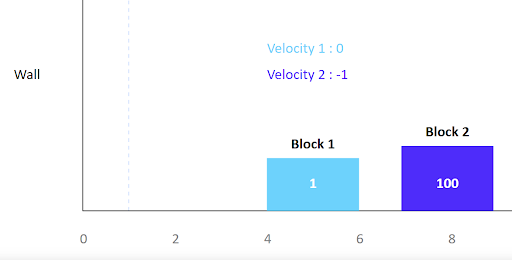
\includegraphics[width=7cm]{liang_1.png}
\end{center}

The answer is that as $N$ increases, the number of collisions begins to resemble, and in fact do match, the digits of $\pi$.

\begin{center}
\begin{tabular}{c|c}
    Mass Ratio & Collisions \\
    \hline
    $1:100^0$ & $3$ \\
    $1:100^1$ & $31$ \\
    $1:100^2$ & $314$ \\
    $1:100^3$ & $3141$ \\
    $1:100^4$ & $31415$ \\
    $1:100^5$ & $314159$ \\
\end{tabular}
\end{center}

Now, one might initially jump to various physics principles to tackle the problem, meticulously calculating individual collisions and formulas. Perhaps a conclusion could be reached after manually calculating different scenarios. However, a better, quite ingenious, method can be found by transforming the problem into a mathematical proof. 

While this relationship seems random, concrete proof exists, first published in 2003 by Gregory Galperin. Though the proof discussed in this article will focus on a more geometric derivation, it relies on the same fundamental concepts as Galperin’s pure math approach. Firstly, the laws of conservation of kinetic energy and momentum must be established, as they are the foundation of a version of this proof. Using the conservation of energy equation $$\frac{1}{2} M {v_M}^2 + \frac{1}{2} m {v_m}^2 = E,$$ we can plot the motion of the system as the points $(v_M, v_m)$, where $v_m$ represents the smaller block's velocity and $v_M$ represents the larger block. At this point, you may recognize that the equation now resembles the standard equation of an ellipse, which does have some sort of connection with pi! But since elliptical circumferences and areas are less directly related to pi than the traditional circle, it really would help to transform the equation to a circle. To remedy this, the equation is rearranged to plot $$(v_M \sqrt{M})^2 + (v_m \sqrt{m})^2 = 2E,$$ which is in the standard form of a circle being $x^2 + y^2 = r^2$.

\begin{center}
    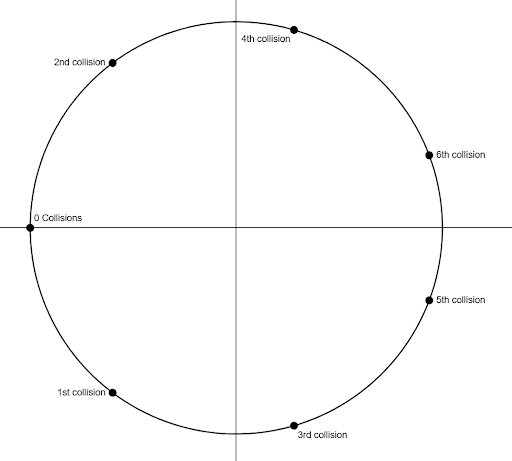
\includegraphics[width=6cm]{liang_2.png}
\end{center}

The circle therefore represents all the possible combinations of velocities of the two blocks that result in the same initial energy, following the law of conservation of energy. We know that there is an initially negative $v_M$ and zero $v_m$, and after the collision occurs some of the energy is transferred to the smaller block. Upon reaching the wall, the velocity of the smaller block is instantly reflected in the opposite direction, resulting in pairs of points of these collisions having the same $x$ values but opposite $y$ values. In order to determine how many collisions there are, however, the number and location of the next coordinates must be determined. By using the conservation of momentum, another equation,
\begin{align*}
    P &= Mv_M + mv_m \\
    &= \sqrt{M}\left(\sqrt{M}v_M\right) + \sqrt{m}\left(\sqrt{m}v_m\right) \\
    &= \sqrt{M} \cdot x + \sqrt{m} \cdot y,
\end{align*}
is derived. From this equation, the slope of the lines connecting the collisions is determined to be $-\frac{\sqrt{M}}{\sqrt{m}}$. As momentum is also conserved in this closed system, the slope of this line would remain constant. Plotting the conservation of momentum equation with the conservation of kinetic energy and calculating the intersections will yield all possible velocity combinations for the given masses; therefore, by counting the number of lines connecting these points, the total number of collisions can be obtained, as any change in the velocities of the blocks can only be attributed to a collision since there are no other factors in the system.

\begin{center}
    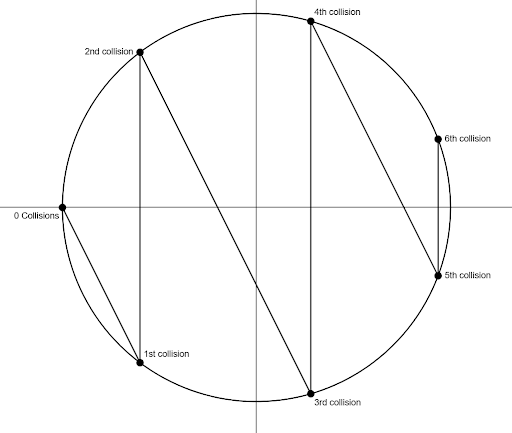
\includegraphics[width=7cm]{liang_3.png}
\end{center}

After this relationship is established, the condition terminating the experiment must be derived---only when both blocks are moving rightward, with the smaller block having a smaller velocity than the larger, will the blocks cease to collide again. Therefore, the final point will be within the region bounded by the line $$y = x\frac{\sqrt{m}}{\sqrt{M}},$$ defining the maximal possible velocities of the smaller block in relation to the larger; the $x$-axis, as both velocities of the blocks must be possible; and the point must be on the graph of the circle given by the first equation. Finally, the number of collisions can be calculated using a clever integration of the inscribed angle theorem, where the intersecting lines creating angle $\theta$ will be an arc length $2\theta$ apart on the intersection of the circle. Since each $2\theta$ arc length corresponds to a singular line, and therefore a collision, the counting question now becomes an issue of how many $2\theta$ segments can be added up before overlapping the circle. As there are $2\pi$ radians in any given circle, then the answer is the inequality $n \cdot \theta < \pi$, where $n$ is the number of collisions.

Proving that the number of collisions results in the digits of pi, a $0.01 = 100^{-1}$ can be substituted for theta, yielding $n=314$, matching the first 3 digits of pi, where the digits will increase as $\theta$ decreases. There exists one issue with this proof, however, and that is that this formula only works for very small values of $\theta$, as it relies on a small-angle approximation of $\theta$ to function. This is because slope, instead of being thought of as $-\frac{\sqrt{M}}{\sqrt{m}}$, can also be rewritten as $\frac{1}{\tan{\theta}}$, yielding $\theta = \arctan{\sqrt{\frac{m}{M}}}$. Therefore, instead of $\theta$ being set to a power of 100, it is rather equal to the arctan of a power of 100, as the ratio of masses will always be a power of 100. As $\arctan{x}$ only approaches $x$ when $x$ is extremely small, the limitation of this proof lies in the fact that there is a chance that solving the inequality with the actual $\theta$ value and arctan of such $\theta$ will yield different results. This remains neither proven nor disproven, though, as current mathematical tools are not equipped to solve such a problem.

If you’re interested in learning more about the interconnectedness of scientific disciplines and math, or this specific problem, I highly encourage you to check out 3Blue1Brown’s Youtube video which includes detailed visualizations, derivations, and explanations of said proof: \url{https://www.youtube.com/watch?v=6dTyOl1fmDo}.
Additionally, you can check out the original, more math-based proof at
\url{https://www.maths.tcd.ie/~lebed/Galperin.%20Playing%20pool%20with%20pi.pdf}.

\end{multicols}

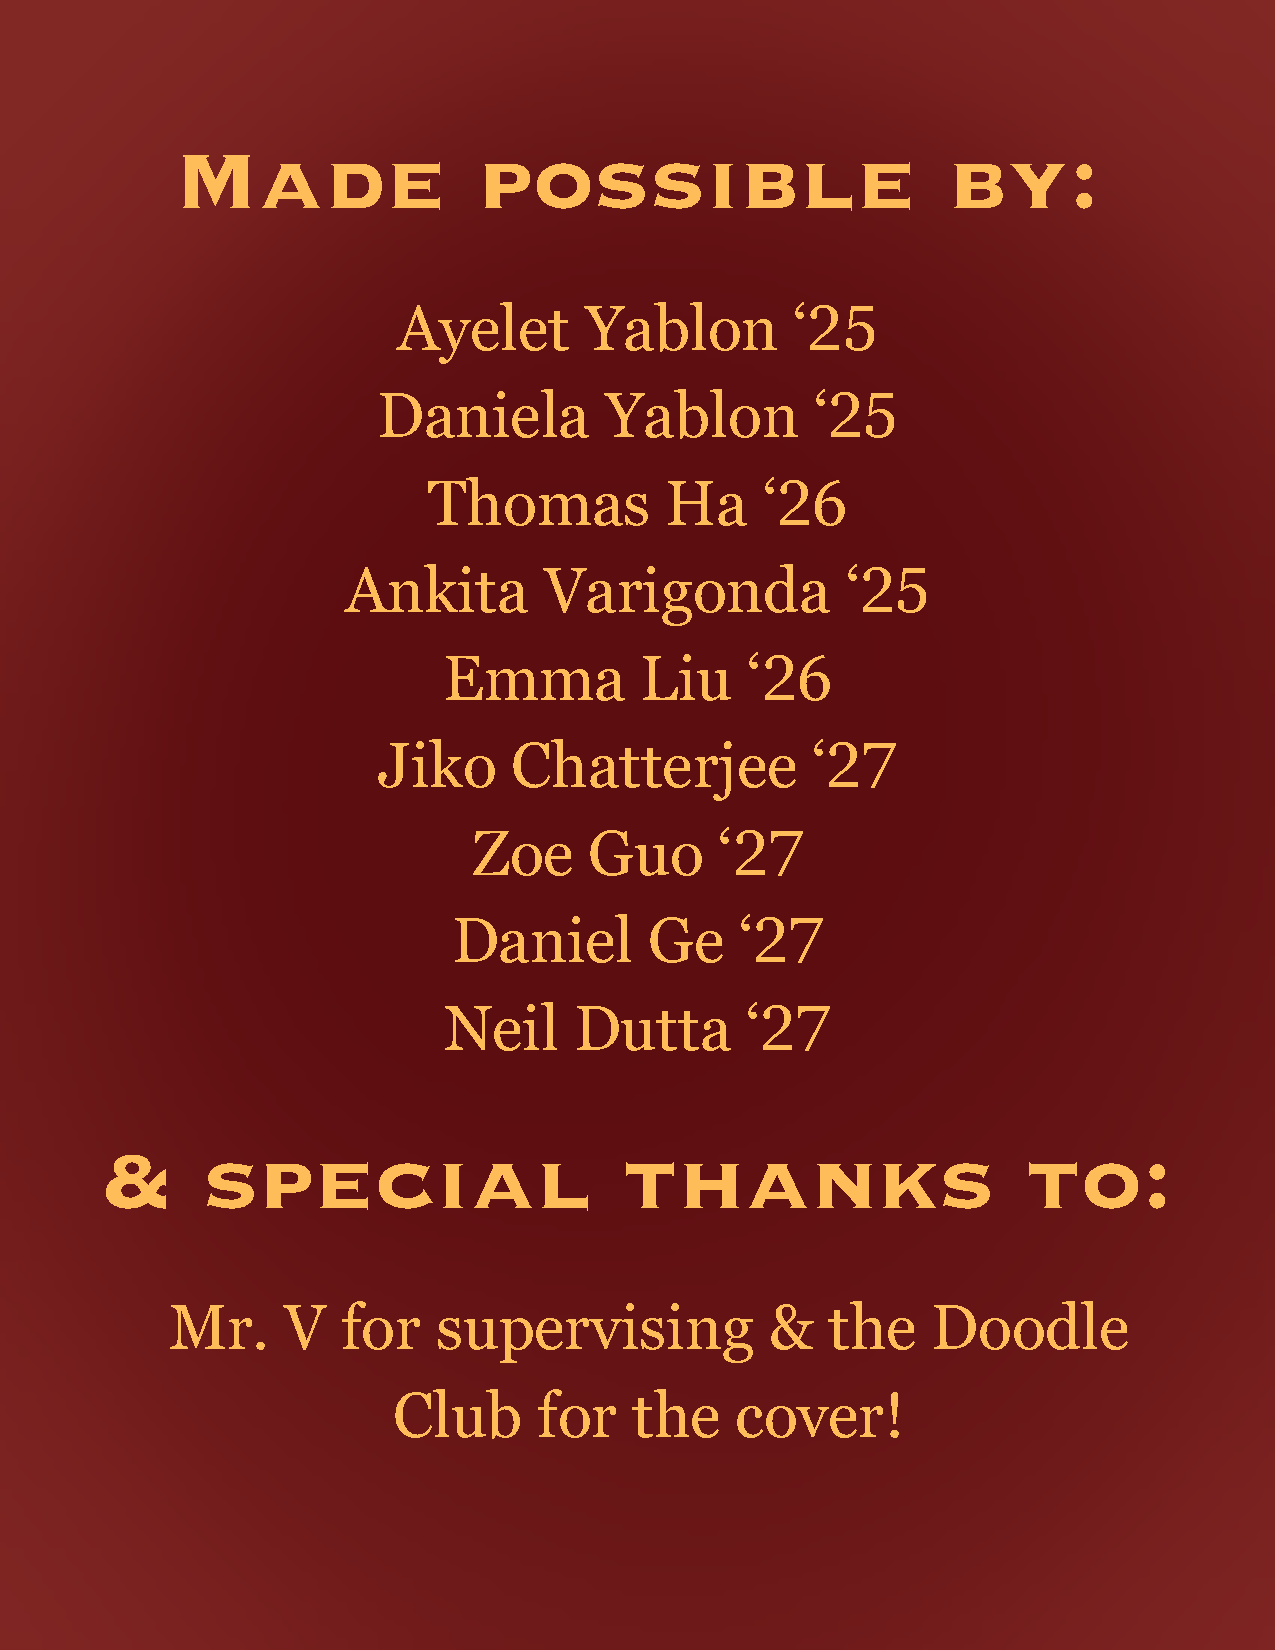
\includepdf{back.pdf}

\end{document}
